
\documentclass{article}
\usepackage{graphicx}
\usepackage{hyperref}
\usepackage{multicol}
\usepackage{verbatim}
\usepackage{biblatex}
\bibliography{citation.bib}

\hypersetup{
	colorlinks=true,
	linkcolor=black,
	filecolor=magenta,      
	urlcolor=blue,
	citecolor=blue,
}
\begin{document}
\begin{titlepage}
	\begin{center}
		\Huge
		\textbf{E-Commerce Relational Database Management System Design}
		
		\vspace{0.5cm}
		\LARGE
		Database Design Project
		
		\vspace{1.5 cm}
		
		\textbf{MD.Owes Quruny Shubho}\\
		\vspace*{0.1cm}
		CSE Graduate\\
		Apprentice Data Scientist\\
		\href{https://www.linkedin.com/in/shubhobd/}{Linkedin}\\
		Email: \href{mailto:owes.shubho@gmail.com}{owes.shubho@gmail.com} 
		
		
		\vspace{1cm}
		
\includegraphics[width=3in]{images/ecommerce_logo.png}
		
		\Large
		Project Link\\
		\href{https://github.com/shubhomedia/Ecommerce_Database_Design/}{Click Here}\\ 
		Dhaka, Bangladesh\\
		16 June 2020\\
		
	\end{center}
\end{titlepage}

	\tableofcontents
	\pagebreak
	\vspace*{2 cm}
	\section{Executive Summary}
	\subsection{Introduction}
	\paragraph{}
		The database is a core component for any dynamic system, In the Ecommerce system there are several subsections that are enabled for running the whole e-commerce system including user, admin, clients, products, delivery system, etc, All parts need to maintain the information and also need to interconnect between them. So A Relational database management system is compulsory for this kind of system. Whatsoever, For many other privileges and accessibility, I chose MySQL as the database management system.
	\subsection{Project Goal}
	\paragraph{}
		Nowadays E-Commerce is one of the hot topics. So I chose this topic to provide a database design for this. In this RDBMS project, I was trying to provide a concept and mid-range to a practical approach to design a Database System that can serve an E-Commerce System.
	\subsection{Functional Description}
	\paragraph{}
		This is a MySQL based database system where I deeply an E-Commerce System Database Components for Better Maintain the e-Commerce data. The system there are 11 tables are provided. Every Table is connecting for a better relational database model and provides hassle-free data management. For Removing data redundancy table relations are maintained as a priority. Every table also indexing enable for better query and giving instant search result.
		\pagebreak
		\vspace*{2 cm}
	\section{Conceptual Model}
	\subsection{Initial Database Model}
	\paragraph{}
		Before final implementation, we should design a conceptual database design that gives us an initial idea about the final database system. This conceptual design, not a final design but it gives us a prototype of the main database system. We can easily design this kind of model online. In my project, I used draw.io online designing too which is a free online designing tool.\\
		\begin{figure}[!h]
			\centering
			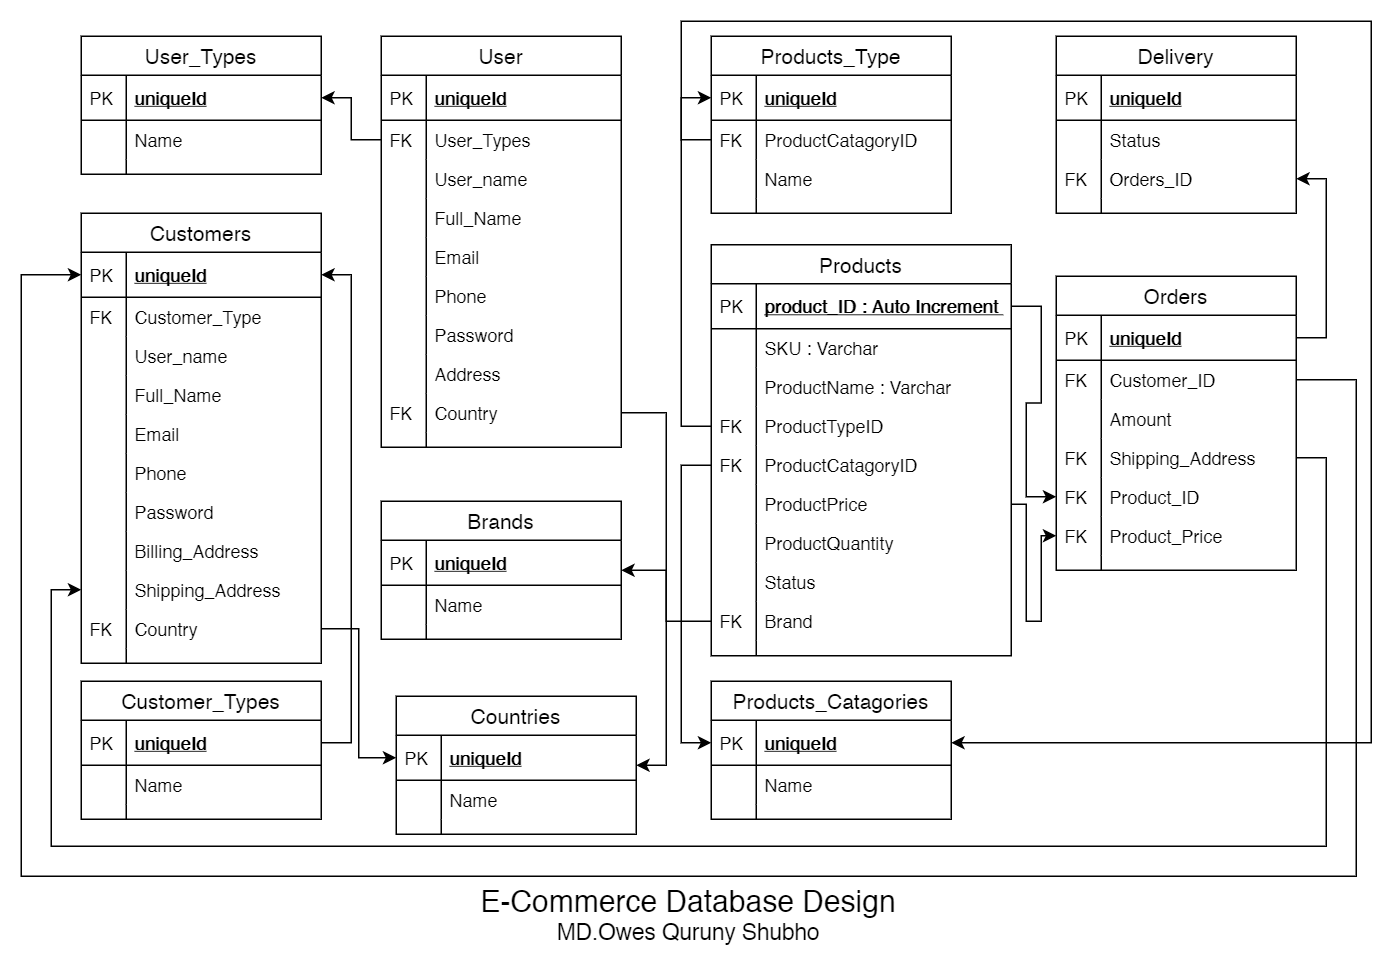
\includegraphics[width=5in]{images/initial_model.png}
			\caption{Prototype of Main Database}
			\label{fig:label}
		\end{figure}
	\pagebreak
	\section{Object Model Diagrams}
	\subsection{Database Tables}
	\paragraph{}
		This database project consist of 11 tables including.
		\begin{center}
			\begin{enumerate}
				\item	Brand
				\item	Country
				\item	Customer
				\item	Customer Type
				\item	Delivery
				\item	Orders
				\item	Product
				\item	Product Category
				\item	Product Type
				\item	User
				\item	User Type
			\end{enumerate}
		\end{center}
	\subsubsection{Brand}
	\paragraph{}
	Brand table is for storing products brands name.
	\subsubsection{Country}
	\paragraph{}
	The country table containing the Country name which is used for Product origin country, user's country, shipment, and customer's shipping address.
	\subsubsection{Customer}
	\paragraph{}
	This table used for storing customer's information. The Customer table containing customer name, Customer username, email address, shipping address, billing Address, also include user password.
	\subsubsection{Customer Type}
	\paragraph{}
	This table used for storing customer type information such as
	Subscribed customer, Pro Customer, etc.
	
	\subsubsection{Delivery}
	\paragraph{}
	Delivery table for Storing information about product delivery and delivery related information
	\subsubsection{Orders}
	\paragraph{}
	Orders table containing order related to all information like order numbers, shipping status, etc.
	\subsubsection{Product}
	\paragraph{}
	Product table for all product related information.
	\subsubsection{Product Category}
	\paragraph{}
	This table contains product category’s like IT, Medical, Books, etc
	\subsubsection{Product Type}
	\paragraph{}
	This table containing product type related information.
	\subsubsection{User}
	\paragraph{}
	This table used for user-related information like user full name, user login id, password, etc
	\subsubsection{User Type}
	\paragraph{}
	This is for user type information, sales manager, accountant or user type information
	\pagebreak
	\subsection{Schema Diagram}
	\paragraph{}
	This schema contains schema objects, which show the tables, columns, data types, views, stored procedures, relationships, primary keys, foreign keys, etc. this database schema can be represented in a visual diagram, which shows the database objects and their relationship with each other
		\begin{figure}[h!]
			\centering
			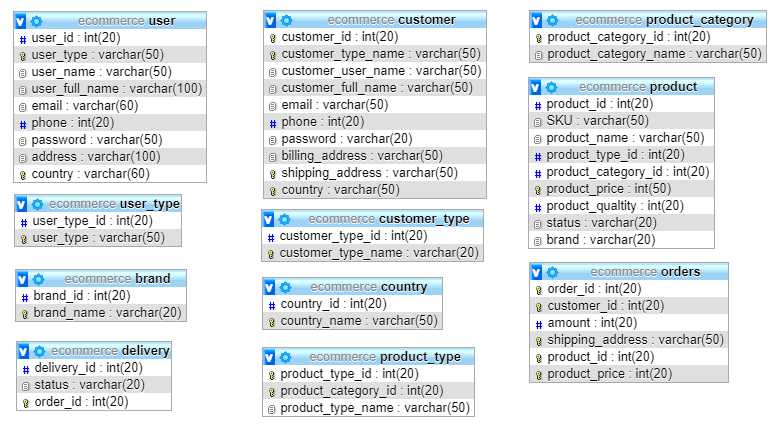
\includegraphics[width=5in]{images/schema_without_relationship}
			\caption{Schema Diagram Without Relationship}
			\label{fig:pic}
		\end{figure}
	\subsection{Database Index}
	\paragraph{}
	This database also has database index enable. this is a data structure that improves the speed of data retrieval operations on a database table at the cost of additional writes and storage space to maintain the index data structure. Indexes are used to quickly locate data without having to search every row in a database table every time a database table is accessed. Indexes can be created using one or more columns of a database table, providing the basis for both rapid random lookups and efficient access of ordered records.
	\pagebreak
	
		\begin{figure}[h!]
			\centering
			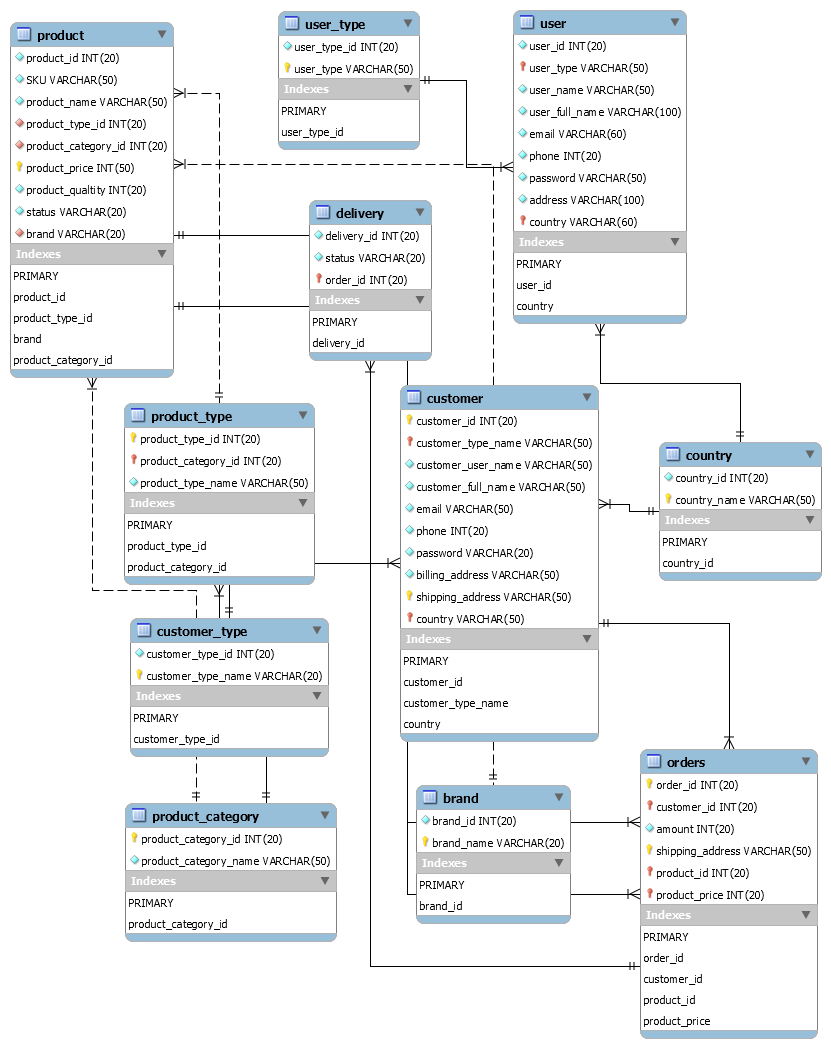
\includegraphics[width=5.3in]{images/schema_with_relationship.png}
			\caption{Schema Diagram With Relationship}
			\label{fig:schema_with_rel}
		\end{figure}
	\pagebreak
	\section{Used Technology}
	
	\begin{itemize}
		\item	\textbf{Conceptual Database Design using Draw.io,\cite{Drawio}}
		\item	\textbf{MySQL Database Ver: 10.1.36- MariaDB,\cite{MySQL} }
		\item	\textbf{MySQL Work bench 8.0 Community Edition,\cite{MySQL_Workbench}}
		\item	\textbf{phpmyadmin 4.8.3,\cite{phpMyAdmin}}
		\item	\textbf{LaTex For Documentation,\cite{LaTex}}
	\end{itemize}
	\section{SQL Statements}
		\subsection{Table Creation}
		\begin{verbatim}
			-- Table structure for table `brand`
			
			CREATE TABLE `brand` (
			`brand_id` int(20) NOT NULL,
			`brand_name` varchar(20) NOT NULL
			) ENGINE=InnoDB DEFAULT CHARSET=utf8;
			
		\end{verbatim}
		
		\begin{verbatim}
		-- Table structure for table `country`
		
		CREATE TABLE `country` (
		`country_id` int(20) NOT NULL,
		`country_name` varchar(50) NOT NULL
		) ENGINE=InnoDB DEFAULT CHARSET=utf8;
		
		\end{verbatim}
		
		\begin{verbatim}
		-- Table structure for table `customer`

		CREATE TABLE `customer` (
		`customer_id` int(20) NOT NULL,
		`customer_type_name` varchar(50) NOT NULL,
		`customer_user_name` varchar(50) NOT NULL,
		`customer_full_name` varchar(50) NOT NULL,
		`email` varchar(50) NOT NULL,
		`phone` int(20) NOT NULL,
		`password` varchar(20) NOT NULL,
		`billing_address` varchar(50) NOT NULL,
		`shipping_address` varchar(50) NOT NULL,
		`country` varchar(50) NOT NULL
		) ENGINE=InnoDB DEFAULT CHARSET=utf8;
		\end{verbatim}
		\pagebreak
		\begin{verbatim}
	-- Table structure for table `customer_type`
	
	CREATE TABLE `customer_type` (
	`customer_type_id` int(20) NOT NULL,
	`customer_type_name` varchar(20) NOT NULL
	) ENGINE=InnoDB DEFAULT CHARSET=utf8;
	
		\end{verbatim}
		
		\begin{verbatim}
		-- Table structure for table `delivery`
		
		CREATE TABLE `delivery` (
		`delivery_id` int(20) NOT NULL,
		`status` varchar(20) NOT NULL,
		`order_id` int(20) NOT NULL
		) ENGINE=InnoDB DEFAULT CHARSET=utf8;
		
		\end{verbatim}
		
		\begin{verbatim}
		-- Table structure for table `orders`
		
		CREATE TABLE `orders` (
		`order_id` int(20) NOT NULL,
		`customer_id` int(20) NOT NULL,
		`amount` int(20) NOT NULL,
		`shipping_address` varchar(50) NOT NULL,
		`product_id` int(20) NOT NULL,
		`product_price` int(20) NOT NULL
		) ENGINE=InnoDB DEFAULT CHARSET=utf8;
		
		\end{verbatim}
		
		\begin{verbatim}
		-- Table structure for table `product`

		CREATE TABLE `product` (
		`product_id` int(20) NOT NULL,
		`SKU` varchar(50) NOT NULL,
		`product_name` varchar(50) NOT NULL,
		`product_type_id` int(20) NOT NULL,
		`product_category_id` int(20) NOT NULL,
		`product_price` int(50) NOT NULL,
		`product_qualtity` int(20) NOT NULL,
		`status` varchar(20) NOT NULL,
		`brand` varchar(20) NOT NULL
		) ENGINE=InnoDB DEFAULT CHARSET=utf8;
		
		\end{verbatim}
		
		\begin{verbatim}
		-- Table structure for table `product_category`
		
		CREATE TABLE `product_category` (
		`product_category_id` int(20) NOT NULL,
		`product_category_name` varchar(50) NOT NULL
		) ENGINE=InnoDB DEFAULT CHARSET=utf8;
		
		\end{verbatim}
		
		\begin{verbatim}
		-- Table structure for table `product_type`
		
		CREATE TABLE `product_type` (
		`product_type_id` int(20) NOT NULL,
		`product_category_id` int(20) NOT NULL,
		`product_type_name` varchar(50) NOT NULL
		) ENGINE=InnoDB DEFAULT CHARSET=utf8;
		
		\end{verbatim}
		
		\begin{verbatim}
		-- Table structure for table `user`

		CREATE TABLE `user` (
		`user_id` int(20) NOT NULL,
		`user_type` varchar(50) NOT NULL,
		`user_name` varchar(50) NOT NULL,
		`user_full_name` varchar(100) NOT NULL,
		`email` varchar(60) NOT NULL,
		`phone` int(20) NOT NULL,
		`password` varchar(50) NOT NULL,
		`address` varchar(100) NOT NULL,
		`country` varchar(60) NOT NULL
		) ENGINE=InnoDB DEFAULT CHARSET=utf8;
		
		\end{verbatim}
		
		\begin{verbatim}
		-- Table structure for table `user_type`
		
		CREATE TABLE `user_type` (
		`user_type_id` int(20) NOT NULL,
		`user_type` varchar(50) NOT NULL
		) ENGINE=InnoDB DEFAULT CHARSET=utf8;
		
		\end{verbatim}
		
		\subsection{Index Creation}
		\begin{verbatim}
			--
			-- Indexes for table `brand`
			--
			ALTER TABLE `brand`
			ADD PRIMARY KEY (`brand_name`),
			ADD KEY `brand_id` (`brand_id`);
			
			--
			-- Indexes for table `country`
			--
			ALTER TABLE `country`
			ADD PRIMARY KEY (`country_name`),
			ADD KEY `country_id` (`country_id`);
			
			--
			-- Indexes for table `customer`
			--
			ALTER TABLE `customer`
			ADD PRIMARY KEY (`customer_id`,`customer_type_name`,`shipping_address`,`country`),
			ADD KEY `customer_id` (`customer_id`),
			ADD KEY `customer_type_name` (`customer_type_name`),
			ADD KEY `country` (`country`);
			
			--
			-- Indexes for table `customer_type`
			--
			ALTER TABLE `customer_type`
			ADD PRIMARY KEY (`customer_type_name`),
			ADD KEY `customer_type_id` (`customer_type_id`);
			
			--
			-- Indexes for table `delivery`
			--
			ALTER TABLE `delivery`
			ADD PRIMARY KEY (`order_id`),
			ADD KEY `delivery_id` (`delivery_id`);
			
			--
			-- Indexes for table `orders`
			--
			ALTER TABLE `orders`
			ADD PRIMARY KEY (`order_id`,`customer_id`,`shipping_address`,`product_id`,`product_price`),
			ADD KEY `order_id` (`order_id`),
			ADD KEY `customer_id` (`customer_id`),
			ADD KEY `product_id` (`product_id`),
			ADD KEY `product_price` (`product_price`);
			
			--
			-- Indexes for table `product`
			--
			ALTER TABLE `product`
			ADD PRIMARY KEY (`product_price`),
			ADD KEY `product_id` (`product_id`),
			ADD KEY `product_type_id` (`product_type_id`),
			ADD KEY `brand` (`brand`),
			ADD KEY `product_category_id` (`product_category_id`);
			
			--
			-- Indexes for table `product_category`
			--
			ALTER TABLE `product_category`
			ADD PRIMARY KEY (`product_category_id`),
			ADD KEY `product_category_id` (`product_category_id`);
			
			--
			-- Indexes for table `product_type`
			--
			ALTER TABLE `product_type`
			ADD PRIMARY KEY (`product_type_id`,`product_category_id`),
			ADD KEY `product_type_id` (`product_type_id`),
			ADD KEY `product_category_id` (`product_category_id`);
			
			--
			-- Indexes for table `user`
			--
			ALTER TABLE `user`
			ADD PRIMARY KEY (`user_type`,`country`),
			ADD KEY `user_id` (`user_id`),
			ADD KEY `country` (`country`);
			
			--
			-- Indexes for table `user_type`
			--
			ALTER TABLE `user_type`
			ADD PRIMARY KEY (`user_type`),
			ADD KEY `user_type_id` (`user_type_id`);
			
		\end{verbatim}
		\pagebreak
		\section{Conclusion}
		\paragraph{}
		To conclude, this project gives us an overview of how an e-commerce systems database we can design. Not just this database design but also, almost every systems need a continuous working process, I also agree that this system not a hindered percent perfect for every e-commerce database.
		
		\section{Future Enhancement}
		\paragraph{}
		In this project I try to provide a 
		database design for an e-commerce system that mainly focus on data relation and data storage.
		In my next project, I will provide some queries and data manipulation statements that fulfill this project. In Future development, I will add some complex queries, table joins, and some triggers.
		\linebreak
		\begin{center}
			\large{THE END, THANK YOU!}
		\end{center}
		\vspace{5cm}
		\printbibliography
		\addcontentsline{toc}{section}{References}
\end{document}